\chapter{実験方法}
\section{概要}
\section{粘度計測}
粘度計測における計測機器の模式図を\ref{fig:viscosity}に示す.ステージと回転する円錐回転子の間に存在する試料によって付加されるトルクを計測することで粘度の計測を行う.粘度のせん断速度依存性を確認することで生成した溶液の性質の確認を行った.なお、計測範囲の都合上、水道水では

\begin{center}
    \begin{figure}[h]
        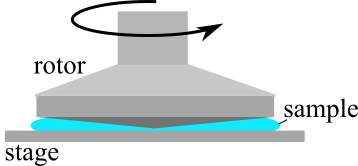
\includegraphics[clip,width=8.0cm]{2-Methods/Viscosity-Measurement.png}
        \caption{Viscosity measurement method.}
        \label{fig:viscosity}
    \end{figure}
\end{center}

\section{球落下実験}

使用した実験装置の概略図を\ref{device}に示す.外寸において高さ255mm,幅50mm,奥行き50mm,厚さ5mmの矩形アクリル水槽に試験溶液を満たした.その上に落下球把持用のピックアップツールをマグネットベースによって固定した.
% TODO:水槽外寸計測
\begin{center}
    \begin{figure}[H]
        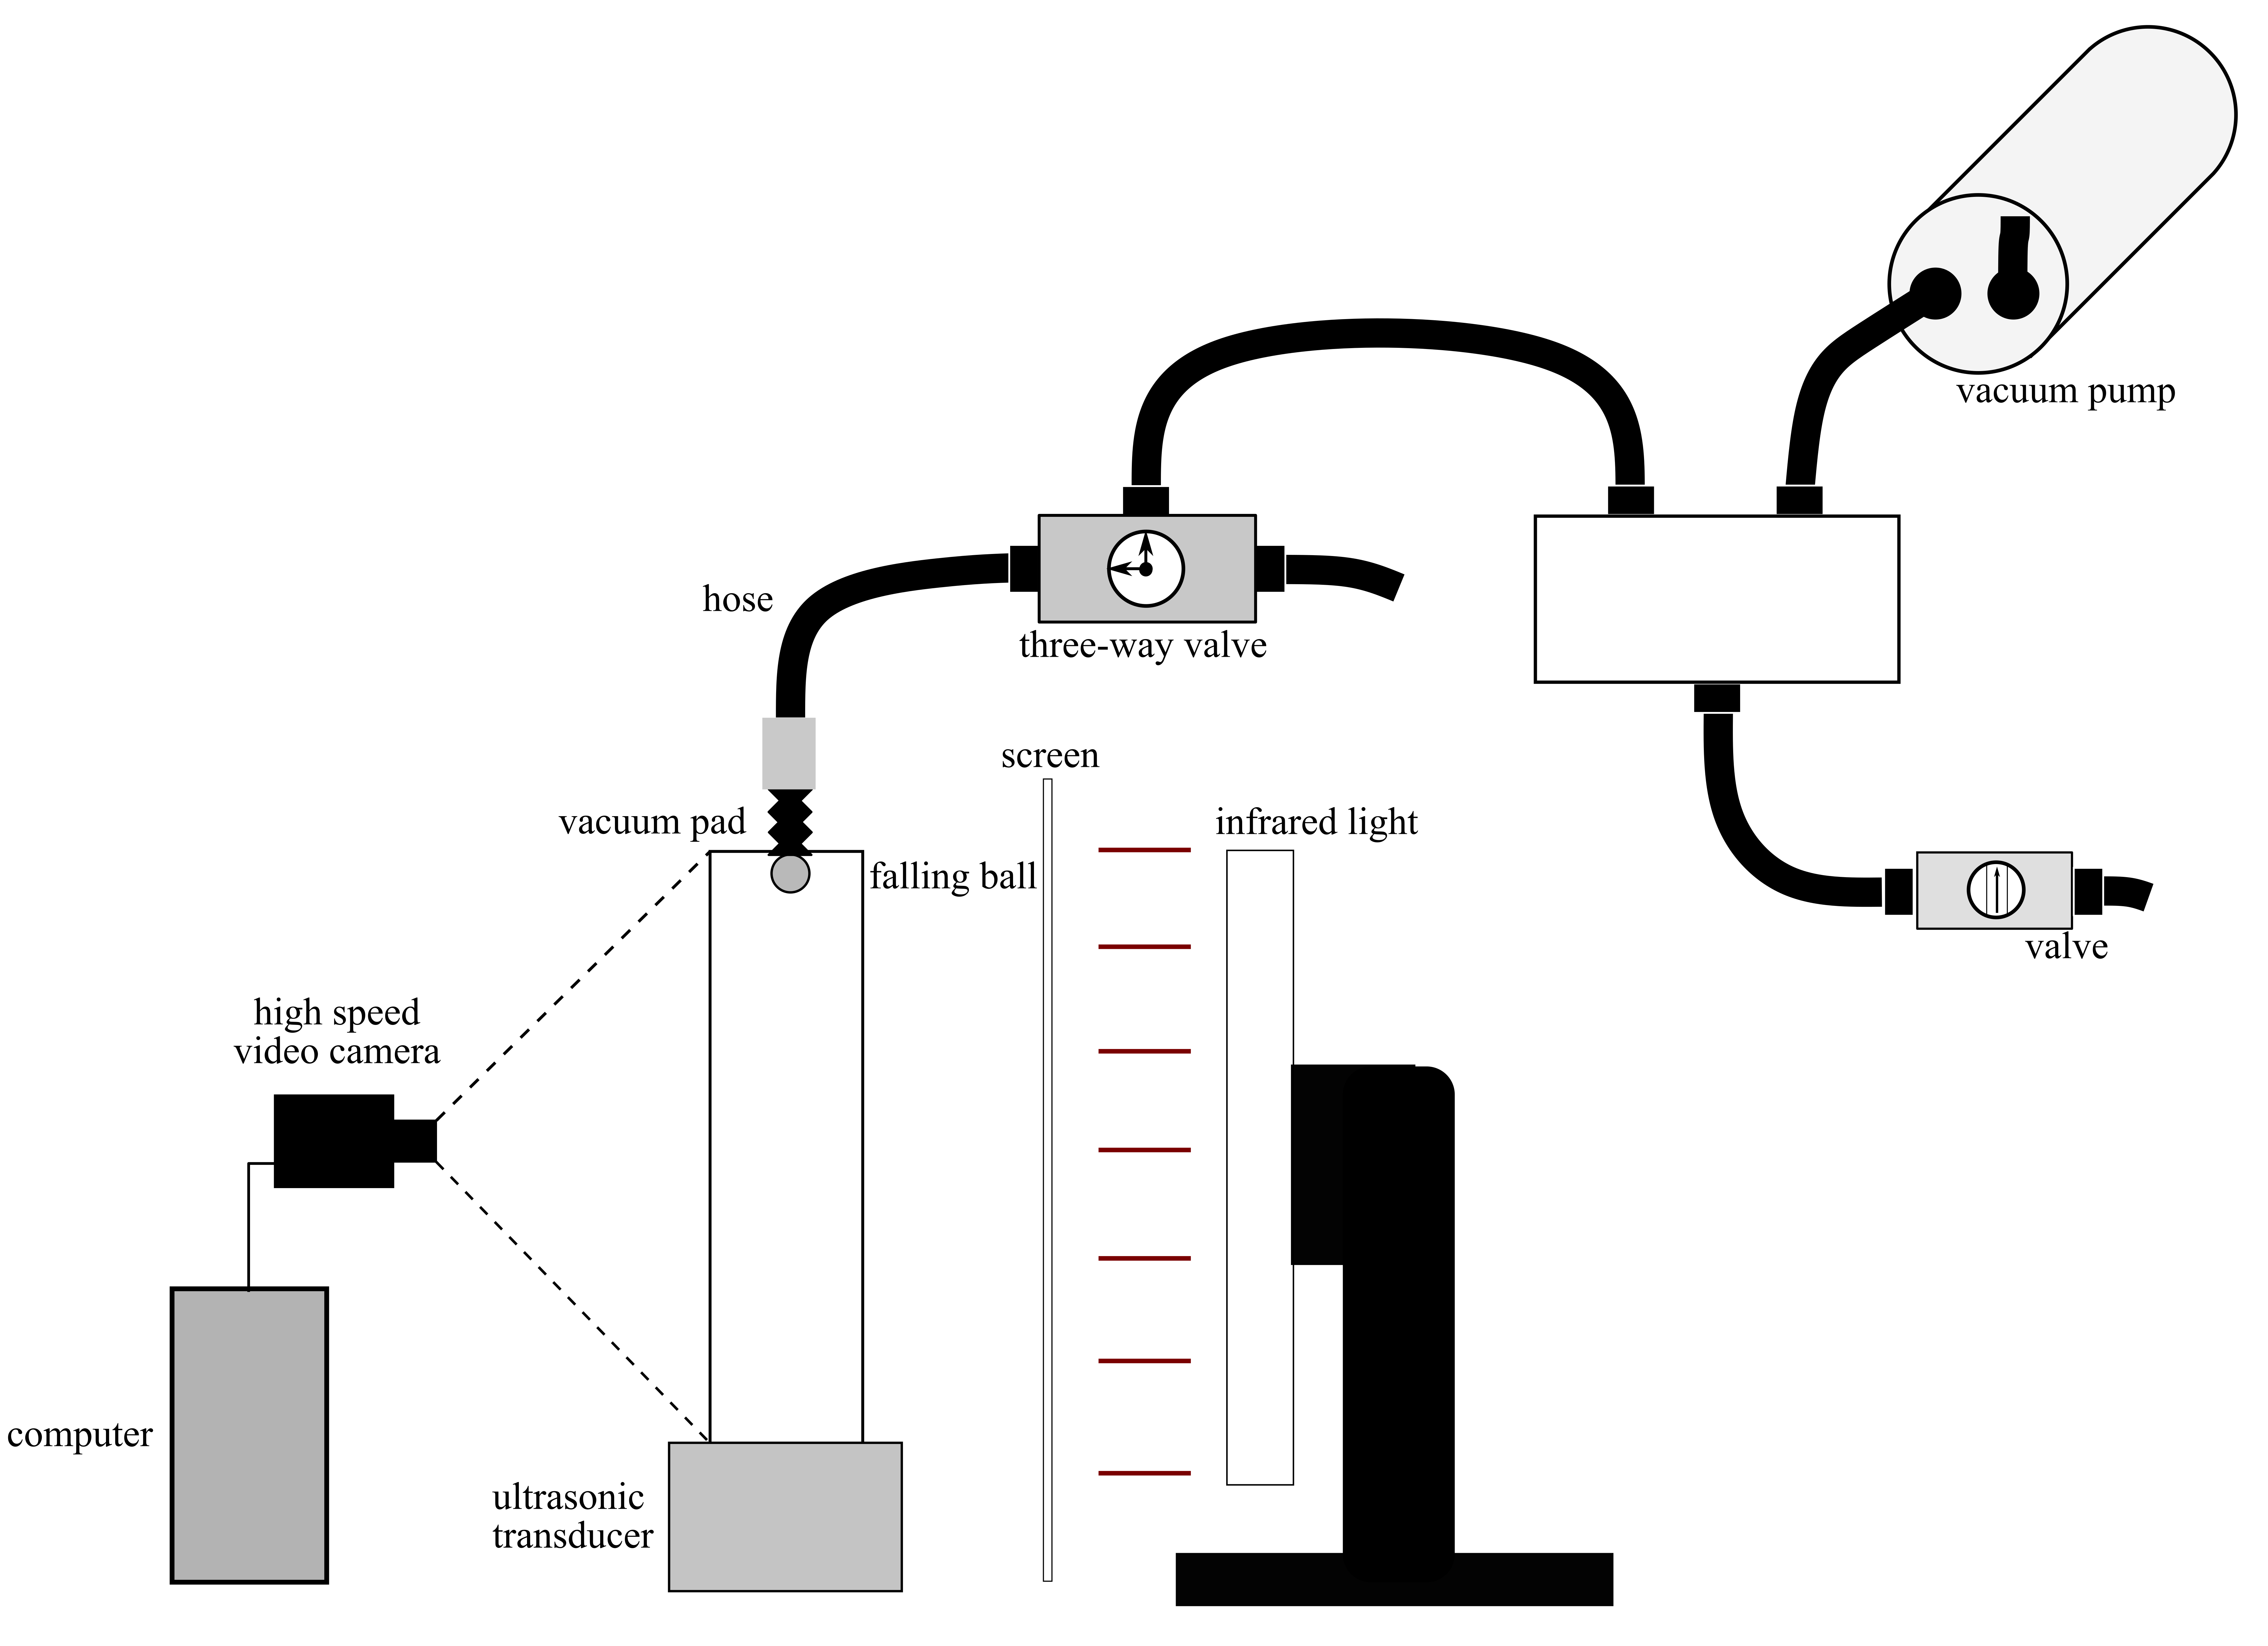
\includegraphics[clip,width=15.0cm]{2-Methods/device.png}
        \caption{Schematic view of the experimental apparatus.}
        \label{fig:device}
    \end{figure}
\end{center}
